% !TeX spellcheck = en_GB
% !TeX TXS-program:compile = txs:///xelatex/[--shell-escape]
% !TeX root = ../build/l2-state-storage.tex




%%%%%%%%%%%%%%%%%%%%%%%%%%%%%%%%%%%%%%%%%%%%%%%%%%%%%%%%%%%%%%%%%%%%%%%%%%%
\section{A zk-Friendly Sparse Merkle Trie for the zkEVM State}

The Merkle tree we are using to store the zkEVM State is a Sparse Merkle Binary Trie fully updatable (that is, allowing both read and write operations)  used to represent key-value data. We will also make it radix in order to optimize storage space. Due to its construction, it will be unbalanced by nature (since keys, which are used to completely locate leaves within the tree, will be hashes of some data).

\paragraph*{Underlying Hash Function}

\texttt{Poseidon} is a cryptographic hash function that has garnered attention for its unique properties and suitability in the context of Zero-Knowledge proofs. It was originally designed to address some of the limitations and challenges faced by traditional hash functions in this specific application domain. From now on, we will consider an instantiation of \texttt{Poseidon} over a Goldilocks field (that is, $\FF_p$ where $p = 2^{64} - 2^{32} + 1$), that takes as entry $8$ field elements divided into two groups: four of them are know as \textbf{capacity elements}, and the other $4$ are the elements to be hashed, known as \textbf{input elements} and outputs $4$ field elements known as \textbf{output elements}. We will denote a Poseidon hash as follows:

\[
\texttt{Poseidon}(\texttt{capacity};\texttt{values})
\]

Here, $\texttt{capacity}$ is an array of $4$ field elements representing the capacity elements, and $\texttt{values}$ is an array of $4$ field elements representing the inputs of the hash. Observe that we can also see \texttt{values} as an array of $8$ (almost) $32$-bits elements. In our context, two instances of Poseidon hash function are employed for protecting the tree against second-preimage attacks: $\texttt{Poseidon}(0; \cdot)$ for branch nodes and $\texttt{Poseidon}(1; \cdot)$ for leaf nodes.


\paragraph*{A Glimpse Through Toy Example}

Let's visualize the tree using an example. Lets suppose we have some set of data associated with four keys: \texttt{000110}, \texttt{001011}, \texttt{001100}, and \texttt{101101}. Prefixes are used to position the leaves containing data. We have four distinct prefixes: \texttt{000}, \texttt{0010}, \texttt{0011}, and \texttt{1}. Recall that zero nodes are used to signify the absence of keys under a given prefix. With this design, similar keys share a common path in the tree, saving space.

\begin{figure}[H]
\centering
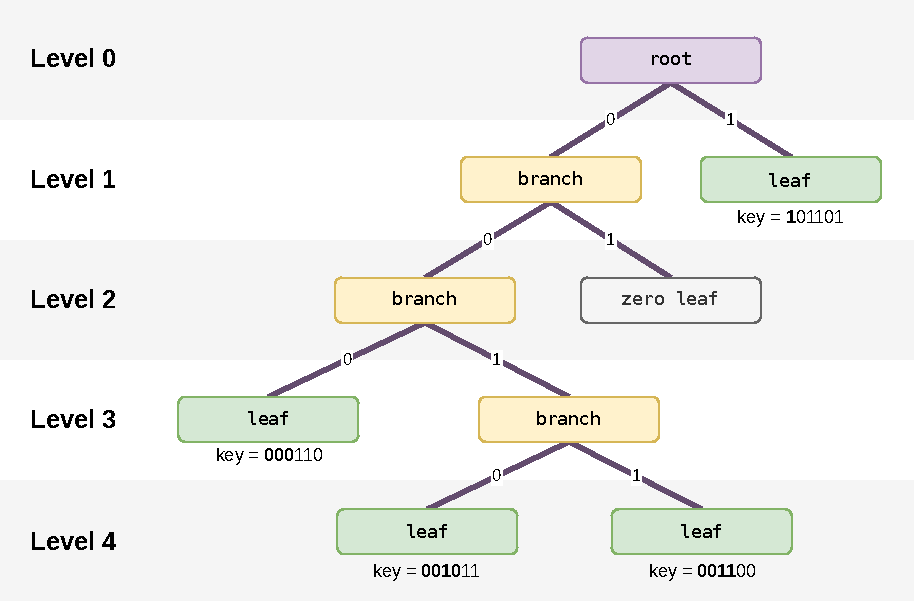
\includegraphics[width=.8\columnwidth]{\zkevmdir/figures/architecture/trie-smt/smt-trie.drawio}
\caption{Illustrative Example of a Sparse Merkle Trie.}
\end{figure}

\paragraph*{The Four Node Types} In the proposed example we can see the $4$ different types of nodes appearing in our tree design:

\begin{itemize}

\item \textbf{Root node}: The root node is the top node of the tree, the only one node at level zero, connecting all branches and leaves. It is the starting point for traversing the tree structure. It serves as a cryptographic summary of all the tree, the final hash of the entire dataset.

\item \textbf{Leaf node}: Leaf nodes encapsulate the actual data associated with a key. Its stored value can be obtained by hashing unique information of each key-value binding of the dataset.

\item \textbf{Branch node}: Branch nodes serve as intermediaries within the tree structure, positioned at various levels between the root node and the leaf nodes. These nodes actively guide the traversal path within the trie. The primary responsibility of a branch node is to store the hash derived from concatenating the hashes of its two child nodes. This hash encapsulates the segment of the cryptographic summary representing the data contained in the subtree rooted at that branch node.

\item \textbf{Zero node}: Zero nodes \textbf{do not} represents a zero value for a specific key. Instead, they denote the absence of a subtree beneath a branch node. In our example, we can see that all keys starting with $01$ share the default value of $0$. Consequently, there is no need for these keys to be individually present as nodes in the tree, and this is where zero nodes come into play. However, the tree actually stores several keys starting with $00$. These keys require the presence of a branch node at level $2$ to obtain the parent's node hash. The optimization lies in the decision not to hash the subtree below with hashes of zero but rather to represent it with an explicit zero value. In practical terms, this means that the branch node at level $1$ assumes a specific value:
\[
\texttt{Poseidon}(0; \texttt{leftChildNode}, 0).
\]

This optimization is called \textbf{partial tree construction}.

\end{itemize}

